\documentclass[usenames,dvipsnames, 18pt, compress, aspectratio=169]{beamer}

% can be compiled by xelatex -shell-escape presentation.tex
% lualatex -shell-escape presentation.tex

\usetheme[]{metropolis}

\usepackage[utf8]{inputenc}
\usepackage[russian, english]{babel}
\usepackage{booktabs}
\usepackage[scale=2]{ccicons}
\usepackage{listings}
\usepackage{marvosym}
\usepackage{color}
\usepackage{xcolor}
\usepackage[document]{ragged2e}
\usepackage[export]{adjustbox}
\usepackage{fontawesome5}
\usepackage{enumitem}
\usepackage{minted}
\usemintedstyle{tango}
\usepackage[normalem]{ulem}
\usepackage{tikz}
\usetikzlibrary{patterns}
\usetikzlibrary{mindmap}
\usetikzlibrary{shapes.misc, fit}
\usetikzlibrary{spy, decorations, decorations.pathmorphing, decorations.pathreplacing, backgrounds, decorations.text}
\usepackage{graphicx}
\usepackage{eso-pic}
\usepackage{verbatim}
\usepackage{smartdiagram}
\usesmartdiagramlibrary{additions}
\usetikzlibrary{trees}
\usepackage{datetime}
\usepackage{hyperref}
\usepackage{forloop}
\usepackage{copyrightbox}
\usepackage{csquotes}
\usepackage{hyperref}
\usepackage{pgfplots}
\usetikzlibrary{tikzmark}
\usetikzlibrary{arrows.meta}

\usepackage{tcolorbox}
\usepackage{tabularx}
\usepackage{array}
\usepackage{colortbl}
\tcbuselibrary{skins}

\usetikzlibrary{shapes,arrows,positioning}
\graphicspath{{images/}}
%\newfontfamily{\FA}{FontAwesome}

\def\social{{\faMastodon}}
\def\github{{\faGithub}}
\def\email{{\faEnvelope}}

\renewcommand{\ttdefault}{pcr}
\setmonofont{FiraCode-VF}
%\newfontfamily{\ttfamily}{FiraCode-VF}

\usefonttheme{professionalfonts} % using non standard fonts for beamer
\usefonttheme{serif} % default family is serif
\usepackage{fontspec}
\setmainfont{Liberation Sans}
\newfontfamily\ExtraLight{Liberation Sans}
\newfontfamily\Light{Liberation Sans}
\newfontfamily\Book{Liberation Sans}
\newfontfamily\Medium{Liberation Sans}

\makeatletter
\newcommand\HUGE{\@setfontsize\Huge{32}{41}}
\makeatother

\newcommand\AtPagemyUpperLeft[1]{\AtPageLowerLeft{%
\put(\LenToUnit{0.85\paperwidth},\LenToUnit{0.05\paperheight}){#1}}}

\newcommand\AtPagemyUpperTop[1]{\AtPageLowerLeft{%
\put(\LenToUnit{0.42\paperwidth},\LenToUnit{0.90\paperheight}){#1}}}

\renewcommand{\ULthickness}{2.0pt}

\definecolor{links}{HTML}{0099FF}
\hypersetup{colorlinks, linkcolor=, urlcolor=links}
\definecolor{greenGood}{HTML}{99FF99}
\definecolor{redBad}{HTML}{FF9980}
\definecolor{title}{HTML}{ee0000}

\setbeamerfont{section title}{family=\Book, size=\Huge, shape=\normalfont}
\setbeamerfont{frametitle}{family=\Book, size=\large, shape=\normalfont}
\setbeamerfont{title}{family=\Book, size=\Large, shape=\normalfont}
\setbeamerfont{subtitle}{size=\small}
\setbeamerfont{author}{family=\ExtraLight, size=\footnotesize}

\definecolor{cec1d24}{RGB}{236,29,36}
\definecolor{cffffff}{RGB}{255,255,255}

\setbeamertemplate{navigation symbols}{}
\beamertemplatenavigationsymbolsempty
\pagenumbering{gobble}

\SetBlockThreshold{0}

\tcbset{
    on line,
    boxsep=4pt,
    left=0pt,
    right=0pt,
    top=0pt,
    bottom=0pt,
    colframe=white
}

\setbeamertemplate{title page}
{

  \vspace*{2.1cm}
  \hspace{6.0cm}
  \begin{minipage}[b][\paperheight]{0.6\textwidth}
  \begin{center}

    \ifx\inserttitle\@empty\else
    {{% \inserttitle is nonempty
      \raggedright%
      %\linespread{1.0}%
      \usebeamerfont{title}%
      \usebeamercolor[fg]{title}%
      %\vspace*{1.3em}
      \if@noSmallCapitals%
        \inserttitle%
      \else%
        \scshape{\color{title} \textbf{\begin{flushleft}\inserttitle\end{flushleft}}}%
      \fi%
      \vspace*{0.3em}
    }}
    \fi

    \vspace*{0.5em}%

    \ifx\insertsubtitle\@empty\else
    {{% \insertsubtitle is nonempty
      \usebeamerfont{subtitle}%
      \usebeamercolor[fg]{subtitle}%
      {\color{black} \insertsubtitle}%
      \vspace*{3.0em}%
    }}
    \fi

    \vspace*{1.0em}%

    \usebeamerfont{author}%
    \usebeamercolor[fg]{author}%
    {\begin{flushleft}\color{black} \insertauthor\end{flushleft}}%

    %\vspace*{1.5em}
    \fontsize{8pt}{10}\selectfont
    {\begin{flushleft}\color{black} 15-12-2022\end{flushleft}}%

    \vfill
    \vspace*{2em}
  \end{center}
  \end{minipage}
}

\setbeamertemplate{section page}
{
  \vspace{2em}
  \centering
  \begin{minipage}{22em}
    \usebeamercolor[fg]{section title}
    \usebeamerfont{section title}
    {\color{black} \insertsectionhead\\[-1ex]}
  \end{minipage}
  \par
}

\setbeamertemplate{footline}
{
\begin{beamercolorbox}[wd=\textwidth,ht=3ex,dp=3ex,leftskip=0.3cm,rightskip=0.3cm]{structure}
  \usebeamerfont{page number in head/foot}
  \insertframenumber
\end{beamercolorbox}
}

\pgfmathdeclarefunction{gauss}{2}{%
  \pgfmathparse{1/(#2*sqrt(2*pi))*exp(-((x-#1)^2)/(2*#2^2))}%
}

\pgfmathdeclarefunction{longtail}{2}{%
  \pgfmathparse{1/(#2*sqrt(2*pi))*exp(-(pow((ln(x)-#1),2))/(2*#2^2))}%
}

\title{Demanding the impossible: \\ rigorous database benchmarking}
\subtitle{}
\date{\today}
\author{DMITRII DOLGOV}
\institute{}

\begin{document}
{
  \usebackgroundtemplate{
\includegraphics[width=\paperwidth]{title.png}}%
  \fontsize{17pt}{18}\selectfont
  \maketitle
}

\AddToShipoutPictureBG{
  \AtPagemyUpperLeft{{
\includegraphics[width=2.0cm,keepaspectratio]{logo.png}}}
}

%\setbeamertemplate{background canvas}{}

\fontsize{17pt}{18}\selectfont

% party tricks references

%{
%\setbeamercolor{background canvas}{bg=black}
%\begin{frame}
    %\frametitle{}
    %\begin{center}
        %\includegraphics[width=1.0\textwidth,center]{nethack.png}
    %\end{center}
%\end{frame}
%\note{Originally about resources, but now not only}
%}

\setbeamertemplate{background canvas}{}

\begin{frame}
    \frametitle{}
    \begin{center}
        Choose your fighter:

        \begin{flushleft}
            \href{github.com/cmu-db/benchbase}{\color{blue!60} github.com/cmu-db/benchbase}
            \href{github.com/akopytov/sysbench}{\color{blue!60} github.com/akopytov/sysbench}
            \href{github.com/brianfrankcooper/YCSB}{\color{blue!60} github.com/brianfrankcooper/YCSB}
            \href{github.com/TPC-Council/HammerDB}{\color{blue!60} github.com/TPC-Council/HammerDB}
            \href{postgresql.org/docs/current/pgbench.html}{\color{blue!60} postgresql.org/docs/current/pgbench.html}

            Replicated live workload
        \end{flushleft}

    \end{center}
\end{frame}

\begin{frame}[fragile]{}
    \frametitle{}
    \begin{center}

		\begin{overprint}[12.5cm]
        \onslide<1>
        \begin{minted}[fontsize=\large]{shell-session}
latency average = 0.011 ms
latency stddev = 0.002 ms
tps = 89357.630697 (without initial connection time)
        \end{minted}

        \onslide<2>
        \begin{minted}[fontsize=\large]{shell-session}
latency average = 0.011 ms
latency stddev = 0.002 ms
tps = 89357.630697 (without initial connection time)

latency average = 0.014 ms
latency stddev = 0.023 ms
tps = 67107.536620 (without initial connection time)
        \end{minted}
		\end{overprint}

    \end{center}
\end{frame}

\section{Benchmarking model}

\begin{frame}
    \frametitle{}
    \begin{center}
        \copyrightbox[b]
        {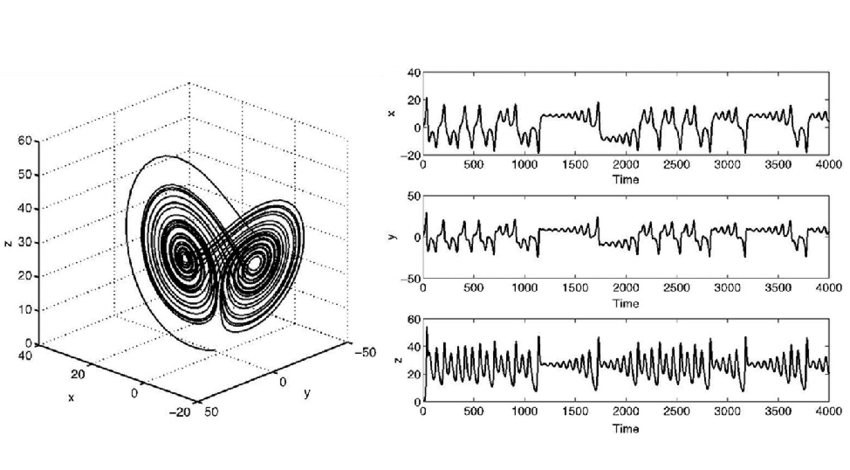
\includegraphics[width=0.8\textwidth,center]{lorenz.png}}
        {
            The phase space plot of the Lorenz attractor,
            \\ {\scriptsize
                \href{https://www.researchgate.net/publication/339796576_Nonlinear_time_series_methods_for_analyzing_behavioral_sequences}
                     {{\color{gray!60} "Nonlinear time series methods for analyzing behavioral sequences"}}}
        }

    \end{center}
\end{frame}

\begin{frame}
    \frametitle{}
    \begin{center}
        Dimentions?

        \begin{itemize}
            \item DB parameters
            \item Hardware resources
            \item Workload parameters
            \item Performance results
        \end{itemize}
    \end{center}
\end{frame}

\begin{frame}
    \frametitle{}
    \begin{center}
        \begin{tikzpicture}
        \begin{axis}[
            grid = major,
            xlabel = shared\_buffers,
            ylabel = queries rate,
            zlabel = query latency,
            xtick = \empty,
            ytick = \empty,
            ztick = \empty,
            ticklabel style = {font = \tiny},
            xmajorgrids=false,
            ymajorgrids=false,
            zmajorgrids=false,
        ]
        \addplot3 [surf, domain=0:180, samples=60]
            { 1 - sin(x) + 0.01 * y };]
        \end{axis}
        \end{tikzpicture}
    \end{center}
\end{frame}

\begin{frame}
    \frametitle{}
    \begin{center}
        \copyrightbox[b]
            {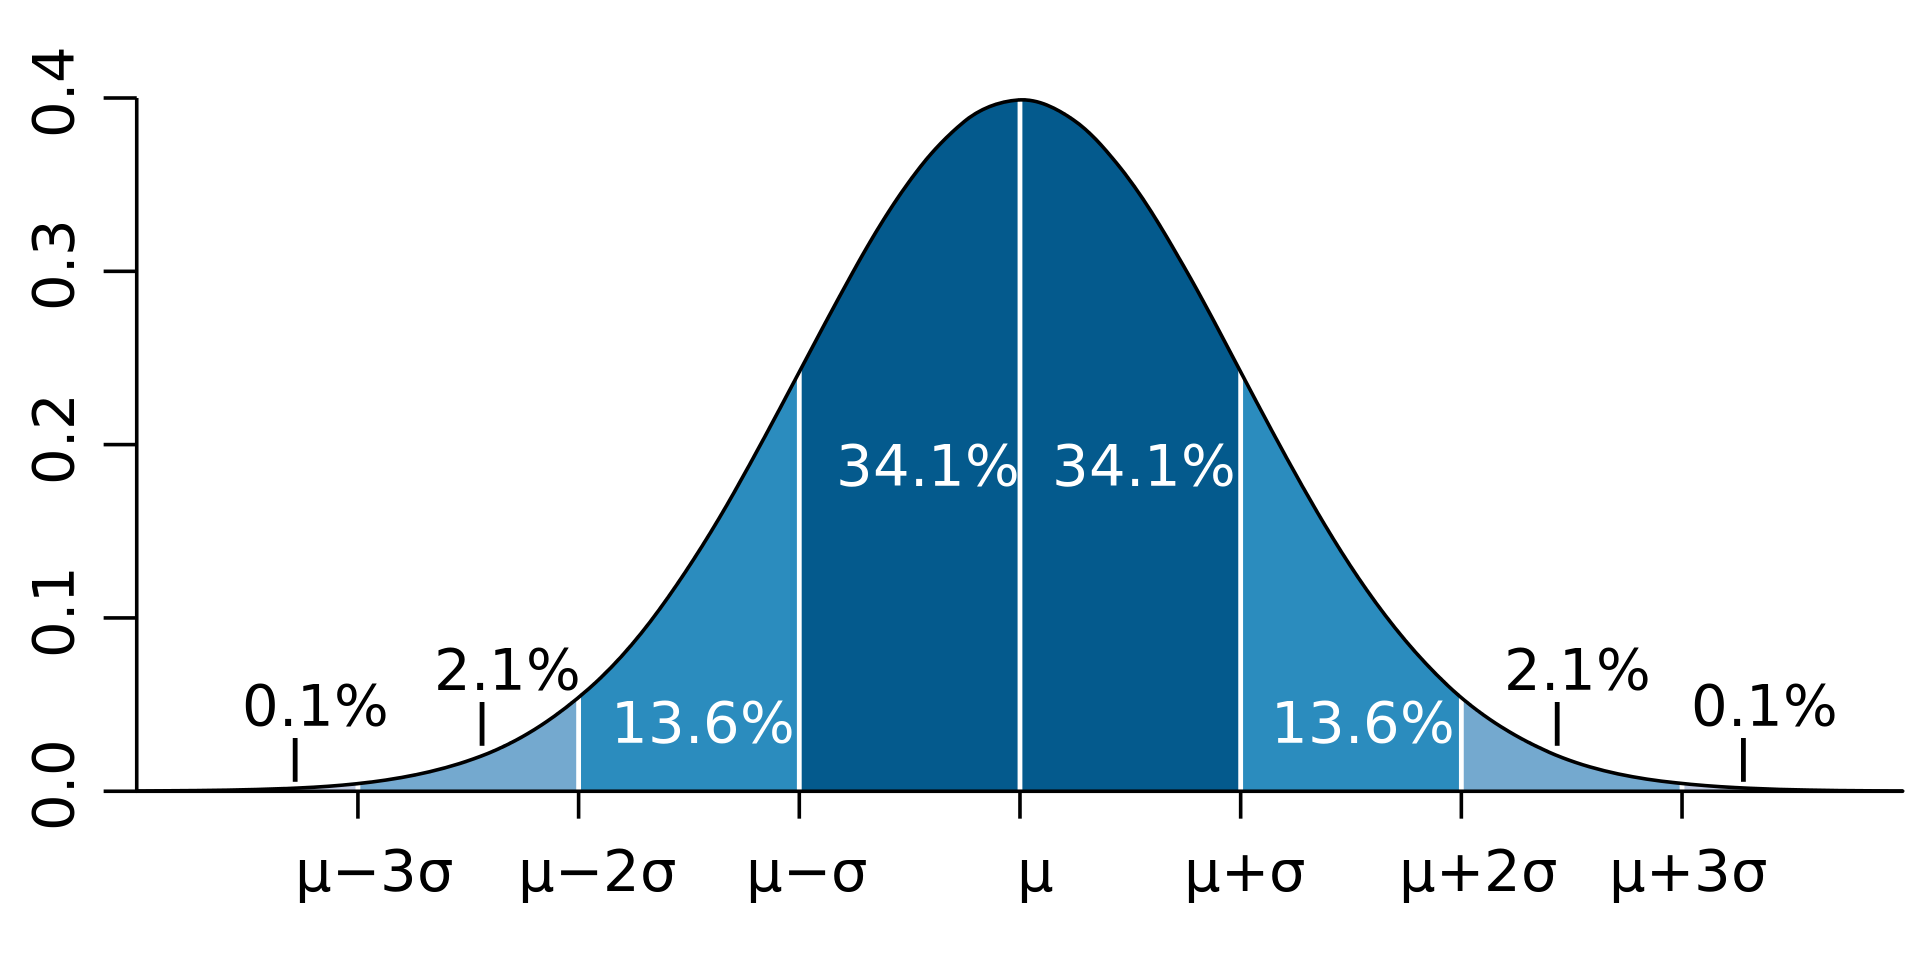
\includegraphics[width=0.8\textwidth,center]{probability-distribution.png}}
            {Probability distribution}

    \end{center}
\end{frame}

\begin{frame}
    \frametitle{}
    \begin{center}
        Benchmarking is exploring the system's {{\bf \tcbox[colback=blue!30]{known}}}
        properties in presence of {\bf {\tcbox[colback=red!30]{unknown}}} factors.

    \end{center}
\end{frame}
\note{
    common vs particular
    statistical approach as clear communication pattern
}

\section{PostgreSQL specifics}

\begin{frame}[fragile]{}
    \frametitle{}
    \begin{center}
        Too low or too high?

        \begin{minted}[fontsize=\large]{shell-session}
    shared_buffers
    max_wal_size
    work_mem
    checkpoint_timeout
    checkpoint_completion_target
    wal_writer_flush_after
    checkpoint_flush_after
    [...]
        \end{minted}

    \end{center}
\end{frame}

\begin{frame}[fragile]{}
    \frametitle{}
    \begin{center}
        Too low or too high?

        \begin{minted}[fontsize=\large]{shell-session}
        vm.nr_hugepages
        vm.dirty_background_bytes
        vm.dirty_bytes
        block/<dev>/queue/read_ahead_kb
        block/<dev>/queue/scheduler
        [...]
        \end{minted}
    \end{center}
\end{frame}
\note{
    fs journal, priorities, etc
}

\begin{frame}[fragile]{}
    \frametitle{}
    \begin{center}
		\begin{overprint}[12.5cm]

        \onslide<1>
        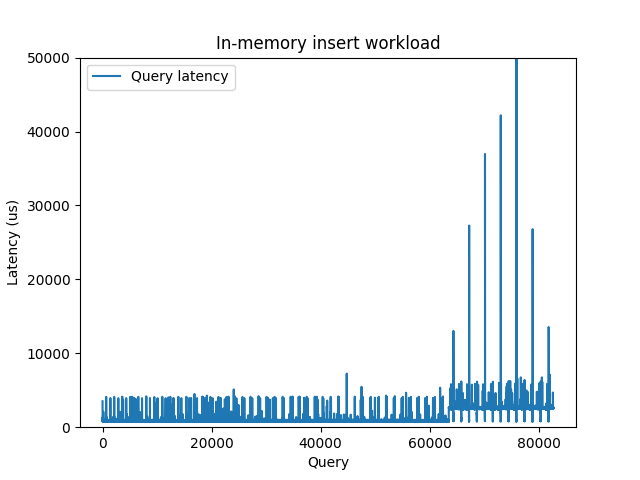
\includegraphics[width=0.8\textwidth,center]{in-memory-insert-latency.png}

        \onslide<2>
        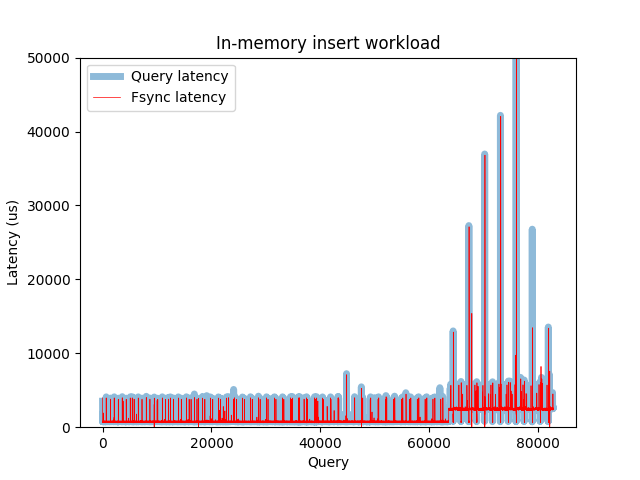
\includegraphics[width=0.8\textwidth,center]{in-memory-insert-latency-sync.png}
		\end{overprint}

    \end{center}
\end{frame}
\note{
    ext4_sync_file_enter/ext4_sync_file_exit
}

%\begin{frame}
    %\frametitle{}
    %\begin{center}
        %Noise, VM, noisy neighbors. hwlat.
    %\end{center}
%\end{frame}

\begin{frame}[fragile]{}
    \frametitle{}
    \begin{center}
        How long?

        \begin{minted}[fontsize=\large]{shell-session}
autovacuum_naptime = 1min
autovacuum_vacuum_threshold = 50
autovacuum_vacuum_insert_threshold = 1000
autovacuum_vacuum_scale_factor = 0.2
autovacuum_vacuum_insert_scale_factor = 0.2
autovacuum_vacuum_cost_delay = 2ms
autovacuum_vacuum_cost_limit = -1
        \end{minted}

    \end{center}
\end{frame}
\note{
    + checkpoints, + bloat
}

\begin{frame}
    \frametitle{}
    \begin{center}
        The load generator?
		\vspace{0.5cm}

		\begin{overprint}[10.0cm]

        \onslide<1>
        \begin{tikzpicture}[thick,scale=1.5, every node/.style={transform shape}]
            % the rectangle with vertical rules
            \draw (0,0) -- ++(2cm,0) -- ++(0,-1.5cm) -- ++(-2cm,0);
            \foreach \i in {1,...,4}
              \draw (2cm-\i*10pt,0) -- +(0,-1.5cm);

            % the circle
            \draw (2.75,-0.75cm) circle [radius=0.75cm];

            % the arrows and labels
            \draw[->] (3.5,-0.75) -- +(20pt,0);
            \draw[<-] (0,-0.75) -- +(-20pt,0) node[left] {$\lambda$};
            \node[draw opacity=0, line width=0, pattern=none, color=white] (generator) at (2.0,1.0cm) {Gen};
            \node at (2.75,-0.75cm) {$\mu$};
            \node[align=center] at (1cm,-2cm) {};
            \node[align=center] at (3cm,-2cm) {};
        \end{tikzpicture}

        \onslide<2>
        \begin{tikzpicture}[thick,scale=1.5, every node/.style={transform shape}]
            % the rectangle with vertical rules
            \draw (0,0) -- ++(2cm,0) -- ++(0,-1.5cm) -- ++(-2cm,0);
            \foreach \i in {1,...,4}
              \draw (2cm-\i*10pt,0) -- +(0,-1.5cm);

            % the circle
            \draw (2.75,-0.75cm) circle [radius=0.75cm];

            % the arrows and labels
            \draw (3.5,-0.75) -- +(20pt,0);
            \draw[<-] (0,-0.75) -- +(-20pt,0) node[left, color=white] {$\lambda$};
            \node (generator) at (2.0,1.0cm) {Gen};
            \draw (generator.west) -| (-20pt, -0.75);
            \draw[<-] (generator.east) -| (4.2, -0.75);
            \node at (2.75,-0.75cm) {$\mu$};
            \node[align=center] at (1cm,-2cm) {};
            \node[align=center] at (3cm,-2cm) {};
        \end{tikzpicture}
		\end{overprint}
    \end{center}

    \linespread{0.5}
    \vspace{0.5cm}
    \color{black}\fontsize{6pt}{0}\selectfont
        "Open versus closed: A cautionary tale". Schroeder, B., Wierman, A. and
        Harchol-Balter, M., USENIX. 2006.
    \linespread{1.5}
\end{frame}
\note{
    The example at the beginning is from pgbench logging vs not logging
}

\section{Statistics}

\begin{frame}
    \frametitle{}
    \begin{center}
        \blockquote{Now any series of experiments is only of value in so far as
            it enables us to form a judgement as to the statistical constants
            of the population to which the experiment belong.}

        \begin{flushright}
            \fontsize{10pt}{0}\selectfont
            Student, 1908. The probable error of a mean. Biometrika, 6(1), pp.1-25.
        \end{flushright}
    \end{center}
\end{frame}

\begin{frame}
    \frametitle{}
    \begin{flushleft}
        Population, metrics

        \begin{center}
        $\mu = E(x)$, $\sigma = \sqrt{E[(X - \mu) ^ 2]}$
        \end{center}

        Samples, statistics

        \begin{center}
        $\overline{X}$, $s_N = \sqrt{\frac{1}{N} \sum^N_{i=1}{(x_i - \overline{x})^2}}$
        \end{center}

        t-test

        \begin{center}
        $t = \frac{\overline{X} - \mu}{\hat{\sigma} / \sqrt{n}}$
        \end{center}
    \end{flushleft}
\end{frame}
\note{
    $\hat{\sigma} -- stddev of mean$
}

\begin{frame}
    \frametitle{}
    \begin{center}
        \begin{tikzpicture}
        \begin{axis}[
            no markers,
            axis lines*=left,
            xlabel=$x$,
            ylabel=$y$,
            every axis y label/.style={at=(current axis.above origin),anchor=south},
            every axis x label/.style={at=(current axis.right of origin),anchor=west},
            height=5cm,
            width=10cm,
            xtick=\empty,
            ytick=\empty,
            enlargelimits=false,
            clip=false,
            axis on top,
            grid = major,
        ]
        \addplot[ultra thick, color=blue, domain=-1:10, samples=100]{gauss(2.5, 1)};
        \addplot[ultra thick, color=red, domain=-1:10, samples=100]{longtail(0, 1)};
        \end{axis}
        \end{tikzpicture}
    \end{center}

    \linespread{0.5}
    \vspace{0.5cm}
    \color{black}\fontsize{6pt}{0}\selectfont
        Hoefler, T. and Belli, R., 2015, November. Scientific benchmarking of
        parallel computing systems: twelve ways to tell the masses when
        reporting performance results. In Proceedings of the international
        conference for high performance computing, networking, storage and
        analysis (pp. 1-12).
    \linespread{1.5}

\end{frame}

\begin{frame}
    \frametitle{}
    \begin{center}
        \blockquote{\it Tests for comparison of means are not affected very much by
            the distributional nonnormality, but this does not extend to the
            comparison of variances.}

        \begin{flushright}
            \fontsize{10pt}{0}\selectfont
            Box, G.E., Hunter, J.S. and Hunter, W.G., 2005. Statistics for
            experimenters. In Wiley series in probability and statistics. Hoboken,
            NJ: Wiley.
        \end{flushright}

    \end{center}

    \linespread{0.5}
    \vspace{0.5cm}
    \color{black}\fontsize{6pt}{0}\selectfont
        Fleming, M., Kolaczkowski, P., Kumar, I., Das, S., McCarthy, S.,
        Pattabhiraman, P. and Ingo, H., 2023, April. Hunter: Using Change Point
        Detection to Hunt for Performance Regressions. In Proceedings of the
        2023 ACM/SPEC International Conference on Performance Engineering (pp.
        199-206).

    \color{black}\fontsize{6pt}{0}\selectfont
        clickhouse.com/docs/en/operations/utilities/clickhouse-benchmark

    \linespread{1.5}

\end{frame}
\note{
    https://github.com/datastax-labs/hunter
    https://clickhouse.com/docs/en/operations/utilities/clickhouse-benchmark
}

\begin{frame}
    \frametitle{}
    \begin{center}
    \end{center}
\end{frame}

\begin{frame}
    \frametitle{}
    \begin{center}
        How much data for confident measurement, ergodic systems.
    \end{center}
\end{frame}

\begin{frame}
    \frametitle{}
    \begin{center}
        Comparing two measurements, factorial design, randomized testing.
    \end{center}
\end{frame}

\section{Final thoughts}

\begin{frame}
    \frametitle{}
    \begin{center}
        Benchmarking = exploring

        known vs unknown

        common vs particular

        validation and verification with other tools \& metrics

        Statistical approach as clear communication pattern
    \end{center}
\end{frame}

\fontsize{18pt}{18}\selectfont
\begin{frame}
  \vspace*{2.5cm}
  \begin{minipage}[b][\paperheight]{\textwidth}
  \begin{center}

      %\raggedright%
      \linespread{1.0}%
      \usebeamerfont{title}%
      \usebeamercolor[fg]{title}%
      \if@noSmallCapitals%
        Questions?
      \else%
        \scshape{\color{black} Questions?}%
      \fi%
      \vspace*{0.3em}

      \usebeamerfont{subtitle}%
      \fontsize{13pt}{14}\selectfont
      \usebeamercolor[fg]{subtitle}%
        \begin{itemize}[label={}]
            \item {\color{black} \social\ @erthalion@fosstodon.org}
            \item {\color{black} \email\ ddolgov at redhat dot com}
        \end{itemize}
      \vspace*{2.5em}%

    \vfill
    \vspace*{2em}
  \end{center}
  \end{minipage}

\end{frame}

\end{document}
